
\documentclass{article}

\usepackage{pgf}
\usepackage{tikz}

\usetikzlibrary{arrows,automata}
\usepackage[latin1]{inputenc}
\begin{document}
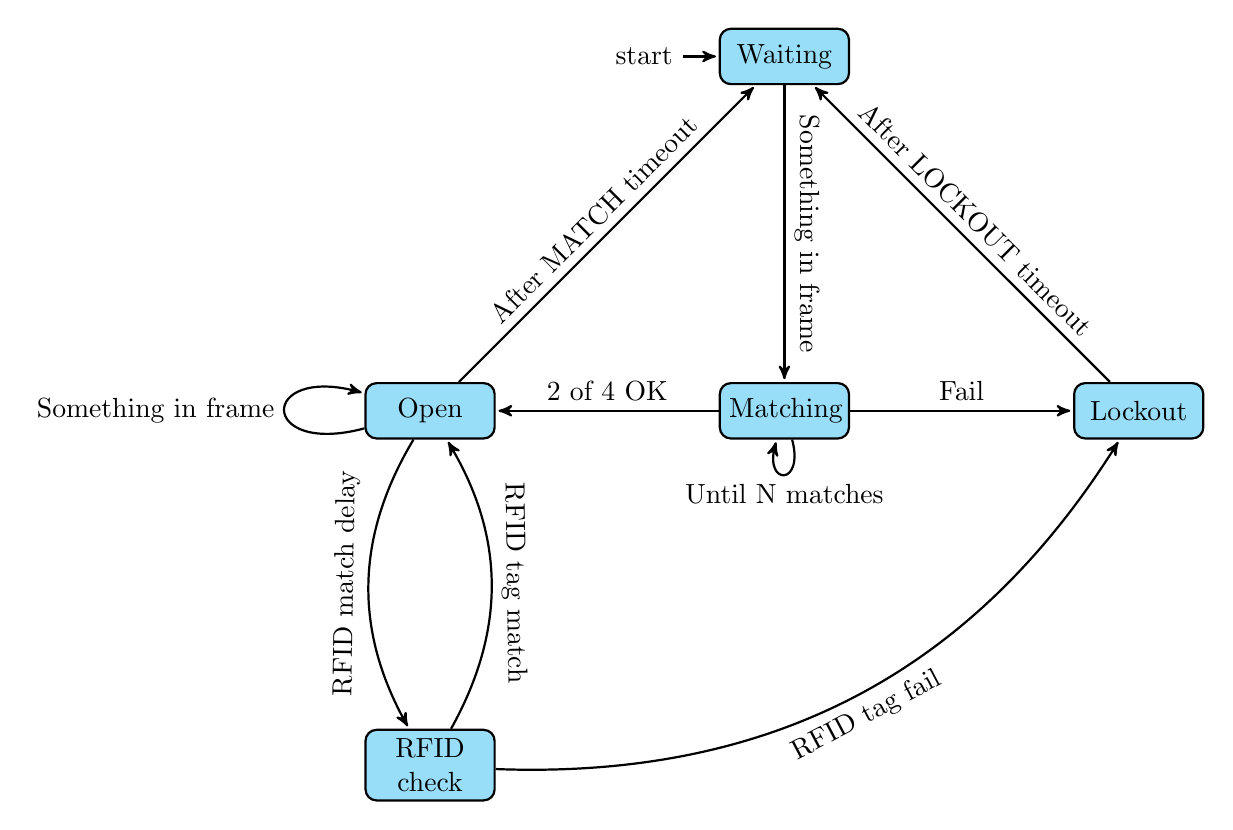
\begin{tikzpicture}[->,>=stealth',shorten >=1pt,auto,node distance=4.5cm,
  thick,main node/.style={circle,fill=blue!20,draw,font=\sffamily\Large\bfseries}]
\tikzstyle{every state}=[fill=red!20,draw=none,text=black]

% Define block styles
\tikzstyle{decision} = [diamond, draw, fill=blue!20, 
    text width=4.5em, text badly centered, node distance=3cm, inner sep=0pt]
\tikzstyle{block} = [rectangle, draw, fill=cyan!40, 
    text width=4em, text centered, rounded corners, minimum height=2em]
\tikzstyle{line} = [draw, -latex']
\tikzstyle{node} = [text height=2em]
\tikzstyle{cloud} = [draw, ellipse, fill=red!20, node distance=3cm, minimum height=2em]

\node[initial,block]	(idle)                    				{Waiting};
\node[block]		(match)	[below of=idle]			{Matching};
\node[block]		(lockout) 	[right of=match]		{Lockout};
\node[block]		(open)	[left of=match]			{Open};
\node[block]		(rfid1)	[below of=open, node distance=4.5cm]	{RFID check};

\path 
	(idle)		edge				node [above, sloped] {Something in frame} (match)
        (match)	edge [loop below]	node {Until N matches} (match)
			edge 			node [above] {2 of 4 OK} (open)
			edge				node {Fail} (lockout)
	(open)	edge [loop left]	node {Something in frame} (open)
			edge				node [above, sloped] {After MATCH timeout} (idle)
			edge	[bend right]	node [above, sloped] {RFID match delay} (rfid1)
	(rfid1)	edge[bend right]	node [above, sloped] {RFID tag match} (open)
			edge	 [bend right]	node [below, sloped] {RFID tag fail} (lockout)
	(lockout)	edge				node [above, sloped] {After LOCKOUT timeout} (idle);

\end{tikzpicture}

\end{document}
